\iffalse
%----------------------------------------------------------------------------------------
%	PACKAGES AND OTHER DOCUMENT CONFIGURATIONS
%----------------------------------------------------------------------------------------
\fi

\documentclass{report}
\usepackage{pstricks, pst-node,pst-tree}
\usepackage{newicktree}
\usepackage{graphicx}
\usepackage{booktabs}
\usepackage{tabularx}
\usepackage{multirow}
\usepackage{xcolor}
\usepackage{hyperref}
\usepackage{ltablex}
\usepackage[a4paper,inner=2cm,outer=2cm]{geometry}
\hypersetup{
    colorlinks,
    linkcolor=black,
    citecolor=red,
    urlcolor=cyan
}

\newcolumntype{b}{X}
\newcolumntype{s}{>{\hsize=.5\hsize}X}

\iffalse
%----------------------------------------------------------------------------------------
%					TITLE PAGE
%----------------------------------------------------------------------------------------
\fi

\newcommand*{\titleGM}{\begingroup
\hbox{
\hspace*{0.1\textwidth}
\rule{1pt}{\textheight}
\hspace*{0.05\textwidth}
\parbox[b]{0.5\textwidth}{

{\noindent\Huge\bfseries Pharmacogenetic Passport}\\[2\baselineskip]
{\large \textit{Pharmacogenetic guidelines and clinical annotations connected to influential DNA changes}}\\[4\baselineskip]
{\large \textsc{ {{json.samplename}} }}\\
{\normalsize \textsc{Creation date: \today}}

\vspace{0.3\textheight}
{\noindent 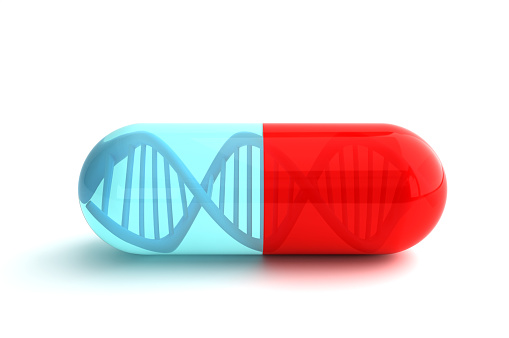
\includegraphics{pilldna}}\\[\baselineskip]
}}
\endgroup}

\iffalse
%----------------------------------------------------------------------------------------
%				BLANK DOCUMENT
%----------------------------------------------------------------------------------------
\fi

\begin{document}

\titleGM

\iffalse
% ------------- TABLE OF CONTENTS -------------------
\fi

\tableofcontents

\newpage

\iffalse
% ----------------  SUMMARY PAGES ----------------------
\fi

\section{Patient haplotypes}

\scriptsize

\begin{tabularx}{\textwidth}{sbb}
\textbf{Gene} & \textbf{Phylogenetic method}\footnote{Method using phylogenetic trees to find closest 'relative' to patient alleles. Trees can be seen in Appendix A.} &  \textbf{Set method}\footnote{Method looking for overlap of haplotype non-reference variants and patient non-reference variants. Reference variants are filtered out of both sets prior to comparison. Top 5 hits can be seen in Appendix 2.}  \\
\hline \\

{{gene.symbol}} & {{gene.new1['1'] }} / {{gene.new2['1'] }} & {{gene.old1['1'] }} / {{gene.old2['1'] }} \\

\end{tabularx}

\normalsize

\newpage

\section{Drug annotations}

\scriptsize
\begin{tabularx}{\textwidth}{bss}
\textbf{Drug} & \textbf{Level 1-2\footnote{ Level 1A and 1B clinical annotations meet the highest levels of criteria and are manually curated by PharmGKB. Level 1A annotations contain a variant-drug combination in a CPIC or medical society endorsed PGx guideline, or, implemented at a PGRN site, or, in another major health system. Level 1B annotations contain a variant-drug combination where the preponderance of evidence shows an association. The association must be replicated in more than one cohort with significant p-values, and, preferably with a strong effect size. Lower levels (3-4) are less significant and may only be based on a single study or case report, which may be performed in vitro.(PHARMGKB) }} & \textbf{Level 3-4\footnote{ See above }}   \\
\hline \\

{{item.drugname}} &  {{item.annCount['1-2'] }} & {{item.annCount['3-4']}} \\

\end{tabularx}

\normalsize

\newpage

\iffalse
% ----------------  Guidelines ----------------------
\fi

\section{Haplotype Guidelines}





\subsection{ {{drug}} }



  
      \subsubsection{ {{gene.genesymbol}} }
     \textit{ {{gene.genename }} } \begin{flushright} \textsc{ {{json.samplename}} \\ {{gene.hapNEW}}  | {{gene.hapOLD}}\footnote{For alternate close matches see Appendix II.} }\end{flushright}
      \hrule \vspace{6pt}
      {{gene.guideline.summary}} \newline
      \scriptsize
      
      \begin{tabularx}{\textwidth}{ {{cols}} }
      {{line}} \\ 
      \end{tabularx}
      
      \normalsize
      
    
  


\newpage

\iffalse
% ----------------  High level Clinical Variations ----------------------
\fi

\section{Clinical Annotations}





\subsection{ {{drug}} }



\subsubsection{ {{gene.genesymbol}} }
\textit{ {{gene.genename}} } \newline


\textbf{\colorbox{red} {Class 1A}} \textbf{ {{ann.rsid}} } \textit{ {{ann.patAllele}} }
{{ann.phenotype}}\newline


\textbf{\colorbox{orange} {Class 1B}} \textbf{ {{ann.rsid}} } \textit{ {{ann.patAllele}} }
{{ann.phenotype}}\newline


\textbf{\colorbox{yellow} {Class 2A}} \textbf{ {{ann.rsid}} } \textit{ {{ann.patAllele}} }
{{ann.phenotype}}\newline


\textbf{\colorbox{green} {Class 2B}} \textbf{ {{ann.rsid}} } \textit{ {{ann.patAllele}} }
{{ann.phenotype}}\newline








\newpage

\iffalse
% ----------------  APPENDICES ----------------------
\fi

\section{Appendix 1: Top 3 haplotypes per gene}
\scriptsize

\begin{tabularx}{\textwidth}{ X | XXXX }
\toprule
\textbf{Gene} & \textbf{Allele 1 (Tree) } & \textbf{Allele 2 (Tree)} & \textbf{Allele 1 (Set) } & \textbf{Allele 2 (Set)} \\
\midrule

{{gene.symbol}}
& {{gene.new1['1']}} & {{gene.new2['1']}} & {{gene.old1['1']}} & {{gene.old2['1']}} \\
& {{gene.new1['2']}} & {{gene.new2['2']}} & {{gene.old1['2']}} & {{gene.old2['2']}}  \\
& {{gene.new1['3']}} & {{gene.new2['3']}} & {{gene.old1['3']}} & {{gene.old2['3']}} \\

\bottomrule
\end{tabularx}
\normalsize
\newpage

\iffalse
% -------------------- LOW LEVEL ANNOTATIONS --------------
\fi

\section{Appendix 3: Low level annotations}

\scriptsize




\subsection{ {{drug}} }




\subsubsection{ {{gene.genesymbol}} }
\textit{ {{gene.genename}} }


\textbf{\colorbox{cyan} {Class 3}} \textbf{ {{ann.rsid}} } \textit{ {{ann.patAllele}} }
{{ann.phenotype}}\newline


\textbf{\colorbox{teal} {Class 4}} \textbf{ {{ann.rsid}} } \textit{ {{ann.patAllele}} }
{{ann.phenotype}}\newline







\end{document}
